\section{Results}

\begin{figure}[h]
    \centering
    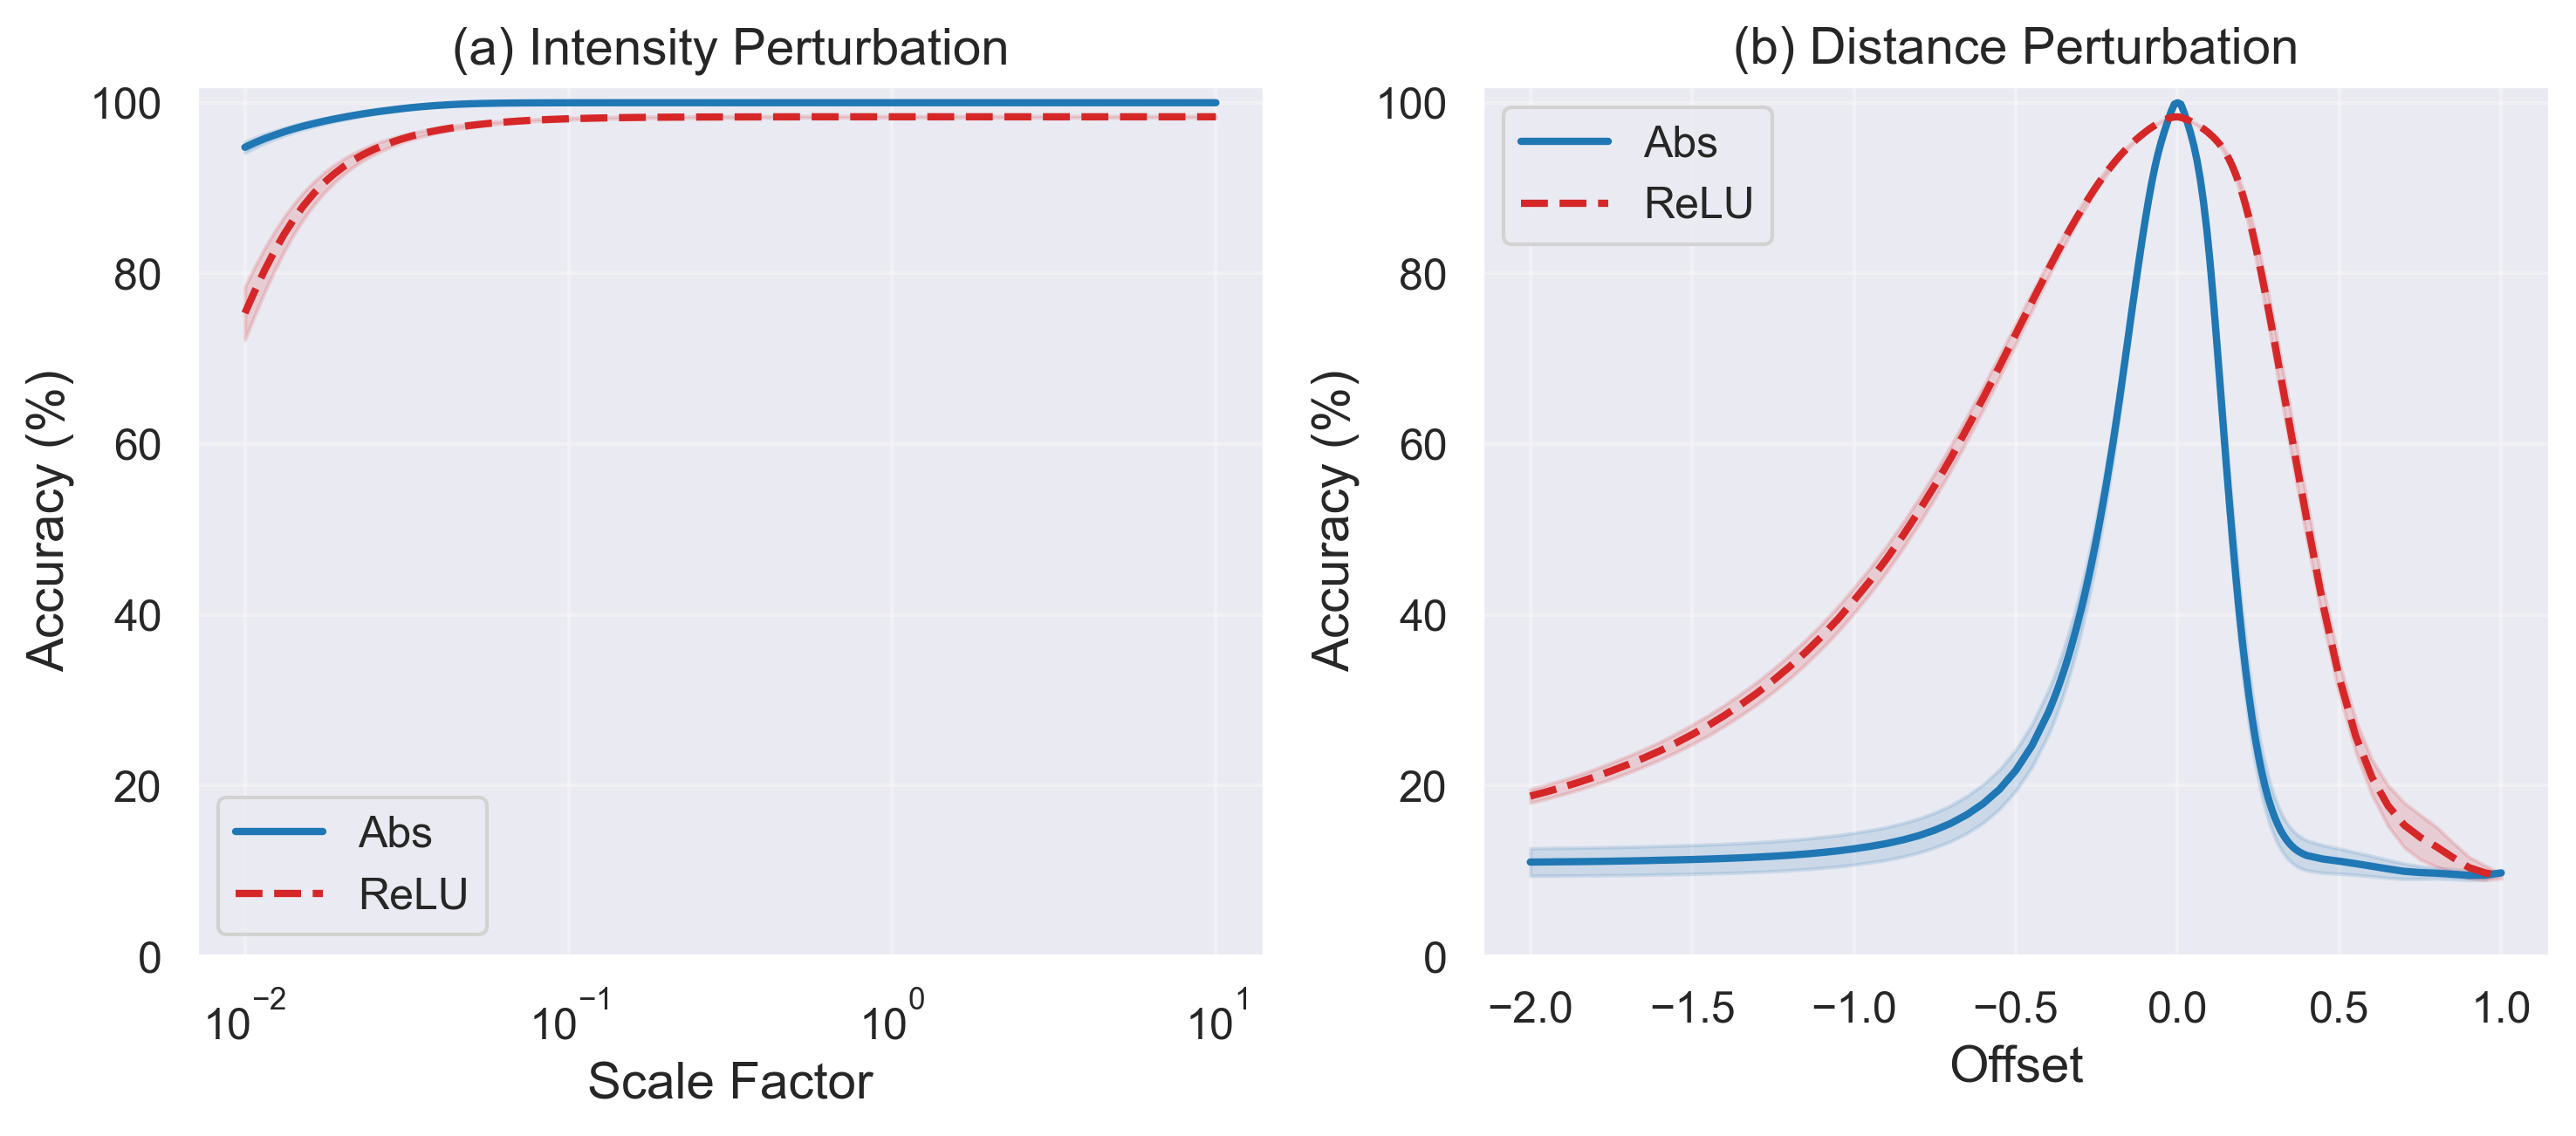
\includegraphics[width=\textwidth]{images/perturbation_analysis}
    \caption{Effects of intensity scaling and distance offset perturbations on model accuracy. Shaded regions represent 95\% confidence intervals across 20 runs.}
    \label{fig:perturbation_analysis}
    \end{figure}
\subsection{Statistical Analysis}   

Results of the experiment provide strong empirical support for our theory that the tested models primarily utilize distance metrics rather than intensity metrics.

Both models achieved strong classification performance on MNIST before perturbation testing, as shown in Table~\ref{tab:baseline}.

Both models demonstrate strong invariance to intensity perturbations while showing significant sensitivity to distance perturbations, supporting our theory. Figure~\ref{fig:perturbation_analysis} shows these effects across perturbation types.

Both models maintain their baseline accuracy (98\% for ReLU and 99\% for Abs) across both scaling (10\% to 200\% of output ranges) and threshold clipping (50\% and above). The minimal drop in performance is small and statisticaly significant (p < 0.01). 

Both models lose accuracy quickly with small offset perturbations. ReLU maintains its baseline of 98\% over a -3\% to +2\% offset range. Abs is even more sensitive and falls below 99\% outside of -1\% to +1\%.

Detailed result statistics, including t-test results are, available in Appendix~\ref{appendix:statistic_tables}.

